\chapter{Design}
    This chapter aims to first extend the concepts of $\Delta$QSD, giving more insights into how the systems need to be instrumented to correctly work together, and how the different parts need to be integrated to interact together.
    \begin{itemize}
        \item We first provide concepts of probes, we extend the $\Delta$QSD notion of failure and describe how time series will work in our oscilloscope, this part is crucial to understand how the different parts of the system work together.
        \item We then split the design of the oscilloscope in two. First explaining the Erlang side, where the system to be tested is. Secondly, we explain the C++ side. Both chapters explain how probes can be inserted and made to work together. We conclude the sections by showing the system diagram of the different parts.
        \item Lastly, we provide high level concepts of the key elements of the oscilloscope. 
    \end{itemize}

    \section{Probes}

To observe the system under test, the resulting outcomes, the result of causal links and outcome expressions, we must put probes in the system. \\
For each outcome of interest, a probe (observation point) is attached to measure the delay of the outcome, like one would in a true oscilloscope. \\
These probes allow to connect the system under test to the stub, which in turns sends a time series of data to the oscilloscope, which performs statistical computations on all the time series. \\
    Consider the figure below, a probe is attached at every component to measure the delay of N outcome ($p_2, p_3$), the stub will send the outcome instance data for each probe observing an outcome to the oscilloscope, which will measure their respective $\Delta$Qs from the time series data and display them (if chosen by the user). \\
    Another probe ($p_1$) is inserted at the beginning and end of the system to measure the global execution delay. \\
    Thanks to this probe, the user can observe the $\Delta$Q \textit{"observed at $p_1$"}, which is the $\Delta$Q which was calculated from the data received by inserting probe $p_1$. The \textit{$\Delta$Q "calculated at $p_1$"} is the resulting $\Delta$Q from the convolution of the observed $\Delta$Qs at $c_2$ and $c_3$.   
    \begin{figure}[H]
        \begin{center}
            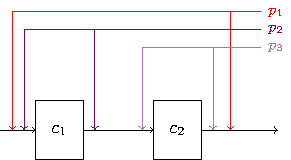
\includegraphics[scale=1.8]{tikz/probes.pdf}
        \end{center}
    \end{figure}

    \section{Extending the notion of failure}
    Whilst previously we defined as "an input message $m_{in}$ that has no output message $m_{out}$", we extend this definition. If you recall the introduction \ref{timeout}, we introduced the notion of a maximum delay.

    We extend the notion of failure to the following definition:
        \begin{center}
            \textit{"An input message $m_{in}$ that has no output message $m_{out}$ after $x$ seconds"}
        \end{center}
    Where $x$ is the $dMax$ defined by the user. We can leverage this new definition to observe $\Delta$Qs in real time.


    \section{Time series - Oscilloscope outcome instances}
    Consider a probe $p$ with two distinct sets of events, the starting set of events $s$ and ending set of event $e$. The outcome instance of a message $m_s \rightarrow m_e$:
    \begin{itemize}
        \item The probe's $p$ name
        \item The start time $t_s$
        \item The end time $t_e$
        \item Its status 
        \item Its elapsed time of execution
    \end{itemize}
    The instance has three possible statuses: \texttt{success, timeout, failure}, it can thus be broken down in the representations, based on its status:
    \begin{itemize}
        \item \textbf{($t_s$,$t_e$)}: This representation indicates that the execution was successful (t $<$ $dMax$). 
        \item \textbf{($t_s, \mathcal{T}$)}: This representation indicates that the execution has timed out (t $>$ $dMax$). The end time and elapsed time is equal to $t_s + \text{timeout}$ 
        \item \textbf{($t_s, \mathcal{F}$)}: This representation indicates the execution has failed given a user defined requirement (i.e. a dropped message given buffer overload in a queue system). It must not be confused with a program failure (crash), if a program crashes during the execution of event $e$, it will time out since the wrapper will not receive an end message.
    \end{itemize}
    The \textbf{time series} of a probe is the sequence of $n$ outcome instances and can then be easily modeled by $\Delta$Q.

    \paragraph{What can be considered a failed execution?} Imagine a queue with a buffer: the buffer queue being full and dropping incoming messages can be modeled as a failure.

    More generally, the choice of what is considered a failed execution is left up to the user who is handling the spans and is program-dependent. Exceptions or errors can be kinds of failure. 

    On another note, the way of handling errored spans in OpenTelemetry can differ from user to user, so the wrapper will not handle ending and setting statuses for "failed" spans.
   

    \section{Application side} 
    
    Before delving deeper into the parts, we present the global system design diagram. We recognise two separate parts, the Erlang side, where the system under test is, and the C++ side, where the $\Delta$Q oscilloscope receives information from the system under test to display graphs.

    \begin{figure}[H]
        \begin{center}
            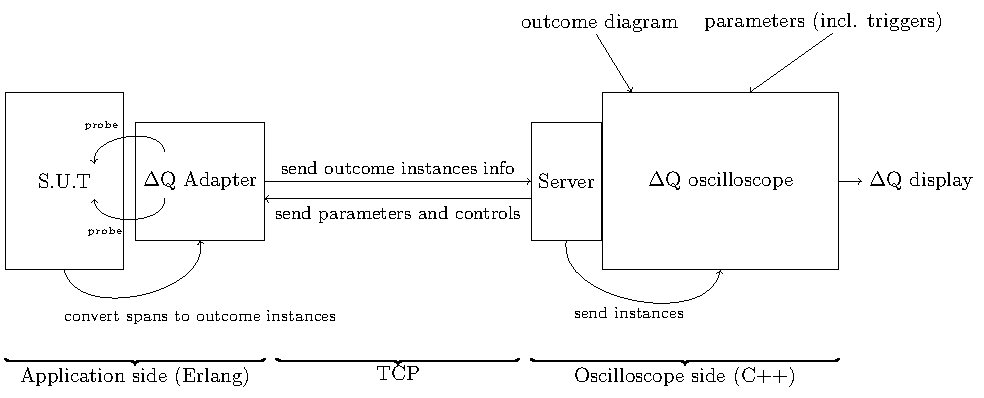
\includegraphics[width=\textwidth]{tikz/sut-stub-osc.pdf}
        \end{center}
        \caption{Global system design diagram.}
    \end{figure}


    \subsection{System under test} The system under test \textbf{(S.U.T)} is the Erlang system the engineer wishes to observe, it ideally is a system which already is instrumented with OpenTelemetry. The ideal system where $\Delta$QSD is more useful is a system that executes many independent instances of the same action \cite{dq-tut}. 
    
    \subsection{$\Delta$Q Adapter} The $\Delta$Q adapter is the \texttt{dqsd\_otel} Erlang application \cite{wrapper}, it starts and ends OpenTelemetry spans and translates them to outcome instances which are useful for the oscilloscope. This can be done thanks to probes being attached to the system under test, like an oscilloscope would! The outcome instances end normally like OpenTelemetry spans or, additionally, can timeout, given a custom timeout ($dMax$), and fail, \textit{according to user's definition of failure}. 
    
    Handling of OpenTelemetry spans which goes beyond starting and ending them is delegated to the user, who may wish to do further operations with their spans. 
    The adapter is called from the system under test and communicates outcome instances data to the oscilloscope via TCP. 
    
    The adapter can receive messages from the oscilloscope, the messages are about updating probe's $dMax$ or starting and stopping the sending of data to the oscilloscope.
    \subsection{Inserting probes in Erlang - From spans to outcome instances}
        OpenTelemetry spans are useful to carry context, attributes and baggage in a program. The plethora of attributes they have is nevertheless too much for the oscilloscope.

        To get the equivalent of spans for the oscilloscope, the adapter needs to be called at the starting events of a probe to start an instance of a probe, and at the ending events to end the outcome instance and send the data to the oscilloscope. The name given with \texttt{"start\_span"} is the name of the probe.

        \begin{minted}{erlang}
        % Start the outcome instance of worker_2 
        {WorkerCtx, WorkerPid} = dqsd_otel:start_span(<<"worker_2">>),   
        % Do work here ...
        %End the outcome instance of worker_2
        dqsd_otel:end_span(WorkerCtx, WorkerPid),
        \end{minted}
  
    \section{Oscilloscope: C++ system}
    \subsection{Server} The server is responsible for receiving the messages containing the outcome instances from the wrapper. The server forwards the instances to the oscilloscope.
    
    \subsection{Oscilloscope} The oscilloscope receives the instances corresponding to probes from the server and adds them to the time series of the probes whose instance is being received. 
    The oscilloscope has a graphical interface which allows the user to create an outcome diagram of the system under test, display real time graphs which show detail about the execution of the system and allow the user to set custom timeouts for probes. It can also display snapshots of the system as if it was frozen in time
 

    \subsection{Inserting probes in the oscilloscope}
        Probes are automatically inserted in the oscilloscope when creating an outcome diagram. They are inserted on the outcomes observables, outcome expressions and to the causal result of outcome expressions, we will see later on how they can be defined and how an outcome diagram can be created. 
        
        In the system below, which is equal to the one defined above, probes are automatically attached to outcomes $o_1, o_2$. The user who wants to observe the result of the sequential composition can insert probes at the start and end of the routine. 

        \begin{figure}[H]
            \begin{center}
                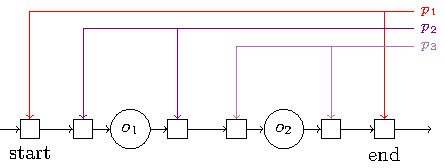
\includegraphics[scale=1.3]{tikz/probe_1.pdf}
            \end{center}
            \label{fig:probes_o}
            \caption{Probes inserted in the outcome diagram of the previous component diagram. \ref{fig:probes}}
        \end{figure}
       
       As for operators (outcome expression), probes are automatically attached to the components inside them and to the start event and end events of the operators. 

       \begin{figure}[H]
           \begin{center}
                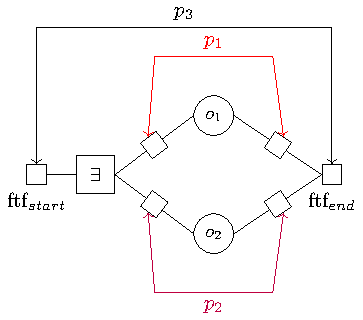
\includegraphics[scale = 1.3]{tikz/probe_2.pdf}
            \end{center}
            \label{fig:probes_op}
            \caption{Probes inserted into an operator.}
       \end{figure}
    
    The \textbf{observed $\Delta$Q} for the first-to-finish operator is the $\Delta$Q from the instances (\textbf{start}, \textbf{end}). The \textbf{calculated $\Delta$Q} is the $\Delta$Q which is the result of the first-to-finish operator being applied on $o_1, o_2$
        


    \section{Oscilloscope system design diagram}
    Now that we have an idea of how all the parts behave together and what they do, we can draw a complete diagram of the interactions of the different components.

    \begin{figure}[H]
    \begin{center}
        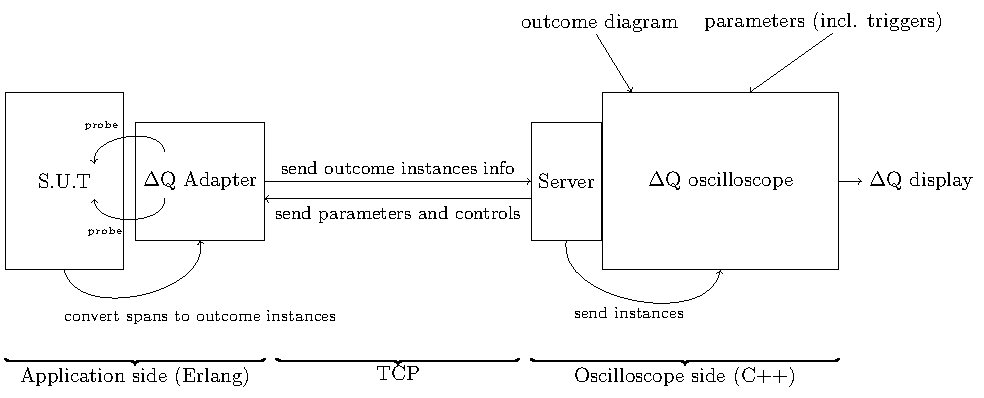
\includegraphics[width=\textwidth]{tikz/sut-stub-osc.pdf}
    \end{center}
    \caption{Global system design diagram.}
    \end{figure}

    \section{Triggers}
    Much like an oscilloscope that has a trigger mechanism to capture periodic signals or investigate a transient event \cite{osc-t}, the \textit{$\Delta$Q oscilloscope} has a similar mechanism that can recognise when an observed $\Delta$Q violates certain conditions regarding required behaviour and record snapshots of the system.

    Each time an observed $\Delta$Q is calculated, it is checked against the requirements set by the user. If these requirements are not met, a trigger is fired and a snapshot of the system is saved to be shown to the user. 
    
    \subsection{Snapshot}
    A snapshot of the system gives insights into the system before and after a trigger was fired. It gives the user a still of the system, as if it was frozen in time. All the $\Delta$Qs which are calculated during the system's execution are stored away. Then, if no trigger is fired, older $\Delta$Qs are removed. Otherwise, the oscilloscope keeps recording $\Delta$Qs without removing older ones, to allow the user to look at the state of the system before and after the trigger.
    

    \section{Polling window}
    To calculate a $\Delta$Q, we take all the outcome instances that ended within a window of time from $t_l$ to $t_u$, a lower and upper time bound.
    
    Suppose we are at time $t$, the window we will display is the  \textbf{window of time $(t-1)_{l}$ - $(t-1)_u$} with $t-1$ equal to $t - x$, and $x$ the polling rate. This is to account for various overheads that need to be taken into consideration, which could be network overhead, the wrapper overhead, C++ latency \dots Imagine multiple outcome instances that are ended at a time slightly lower but close to t, and due to the overheads the messages arrives at a time slightly higher but close to t, the outcome instance would not be taken into consideration for the calculation of a $\Delta$Q.
    
    \begin{figure}[H]
        \begin{center}
            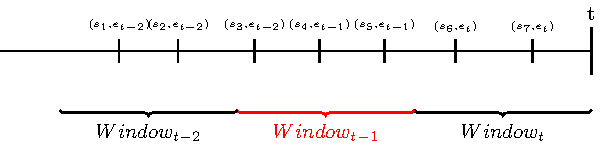
\includegraphics{tikz/window.pdf}
        \end{center}
    \end{figure}

    The polling window then advances every $x$ seconds setting the new window: 
    \begin{center}
        From: $(t-1)_l$, $(t-1)_u$ $\xrightarrow{t + 1}$ $t_l, t_u$. \\
        Where: $t_l = (t-1)_u$ and $t_u = (t-1)_u + x$ 
    \end{center}

